\chapter{Periodic Task Scheduling}
\textit{Scheduling} di \textit{tasks} \textbf{periodici} o \textbf{sporadici} (\textbf{aperiodici}). Definiamo un \textbf{task periodico} $\tau_i(C_i, T_i)$ con $C_i$ il \textit{worst case execution time} e $T_i$ il \textbf{periodo} per il quale il task $\tau_i$ deve essere eseguito.
\begin{figure}[h]
    \centering
    \begin{minipage}[t]{0.45\textwidth}
        \centering
        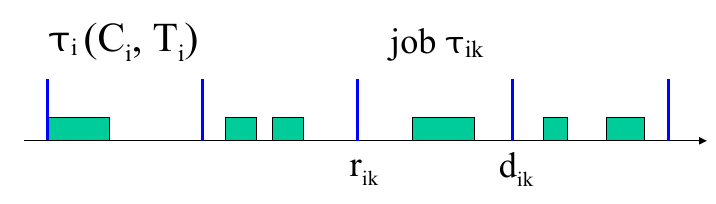
\includegraphics[width=\textwidth]{img/T_aT}
        \caption{\textit{periodic task}}
    \end{minipage}
    \begin{minipage}[t]{0.45\textwidth}
        \centering
        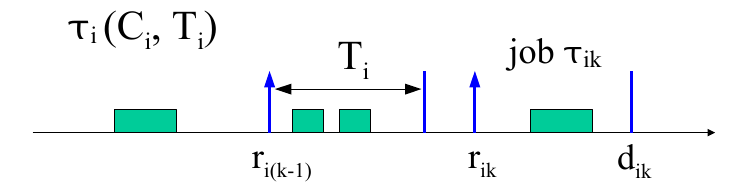
\includegraphics[width=\textwidth]{img/T_aT_1}
        \caption{\textit{sporadic task}}
    \end{minipage}
\end{figure}
\\
Per ogni task periodico, bisogna garantire che:
\begin{itemize}
    \item ogni job $\tau_{ik}$ venga attivato in $r_{ik} = (k - 1) \cdot T_i$.
    \item ogni job $\tau_{ik}$ completi la sua esecuzione entro $d_{ik} = r_{ik} + D_i$.
\end{itemize}
Anche nel caso di \textbf{task aperiodici} possiamo definirli $\tau_i(C_i,T_i)$, in questo caso però $T_i$ non è il periodo nel quale per il quale si ripete il task ma indica il \textit{deelay} minimo di attivazione tra un task $\tau_{ik}$ e un task $\tau_{i(k+1)}$, infatti bisogna garantire per ogni task sporadico che:
\begin{itemize}
    \item ogni job $\tau_{ik}$ viene attivato in un istante $r_{ik} \geq r_{i(k-1)} + T_i$.
    \item ogni job $\tau_{ik}$ completi la sua esecuzione entro una \textit{deadline} relativa $d_{ik} = r_{ik} + D_i$
\end{itemize}

\section{Timeline Scheduling}
È una tipologia di \textit{scheduling offline} è stata utilizzata per anni nei contesti in cui era richiesto un \textit{hard real time} per via della delicatezza delle circostanze di uso (sistemi militari, navigazioni e sistemi di monitoraggio). Può essere chiamato anche \textbf{\textit{cycle executive}} o \textbf{\textit{cyclic scheduling}}. \\
Il funzionamento era tale che l'asse del tempo venisse divisa in intervalli con lunghezza uguale, anche chiamati \textbf{\textit{time slots}}, ogni task viene allocato staticamente in un certo slot e in un certo ordine per venire incontro ai \textit{request rate} desiderati. L'esecuzione per ogni slot viene attivato tramite un \textbf{\textit{timer}}. Consideriamo un task set $\mathcal{T} = \{\tau_1, \tau_2, ..., \tau_k\}$ e che $\forall \tau_i \in \mathcal{T} \; \exists (C_i, T_i)$, in questo caso $T_i \equiv D_i$ ovvero che il periodo del task corrisponde con la sua \textit{deadline} assoluta. Definiremo:
\begin{itemize}
    \item il \textbf{\textit{minor cycle}} come $\Delta = gcd(T_i, T_j) \; \forall T_i, T_j \in \mathcal{T}, \; i \neq j$
    \item il \textbf{\textit{major cycle}} come $\mathbf{T} = lcm(T_i, T_j) \; \forall T_i, T_j \in \mathcal{T}, \; i \neq j$
    \begin{itemize}
        \item nel caso in cui ci siano task sporadici come andiamo a valorizzare il \textit{major cycle}
    \end{itemize}
\end{itemize}
\begin{figure}[h]
    \centering
    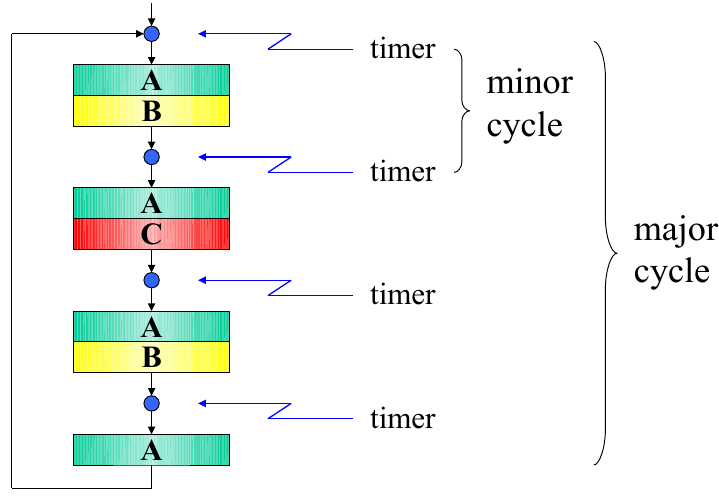
\includegraphics[width=0.5\textwidth]{img/ts}
\end{figure}
\begin{tabular}{ p{7.25cm} | p{7.25cm} }
    \textcolor{green}{\textbf{Vantaggi}} & \textcolor{red}{\textbf{Svantaggi}} \\
    \textbf{-} implementazione semplice (non viene richiesto alcun sistema operativo \textit{real-time}) &  \textbf{-} non è robusto contro \textit{overload} del sistema \\
    \textbf{-} ogni procedura condivide un \textit{address space} comune & \textbf{-} nel caso di aggiunta di un nuovo task è molto difficile l'espansione dello \textit{scheduler} \\
    \textbf{-} basso \textit{overhead} a tempo di esecuzione & \textbf{-} non è facile gestire task aperiodici \\
    \textbf{-} permette di controllare i \textit{jitter} & \textbf{-} tutti i processi devono avere periodo multiplo del \textit{minor cycle} \\
     & \textbf{-} è difficile includere processi con un periodo lungo \\
     & \textbf{-} difficile da costruire e da mantenere \\
     & \textbf{-} tutti i processi con un \textit{WCET} variabile devono essere \textit{splittati} in procedure con lunghezza fissa. (il determinismo non è richiesto, ma la predicibilità si) \\
\end{tabular}
\\ \newline
Durante un \textbf{\textit{overload}} si possono ``considerare'' due vie: la prima è quella di lasciar finire il task, che però comporta un \textbf{effetto domino} che va a portare delle ripercussioni anche su tutti gli altri task e che potrebbe portare ad un \textbf{\textit{timeline break}}; il secondo caso è gestire l'\textit{overload} con l'interruzione del task, in questo caso il sistema potrebbe rimanere in uno stato \textbf{inconsistente}. In un altro caso si ha necessità di incrementare il \textit{WCET} di un task, ma se al somma dei \textit{WCET} dei task in esecuzione nel $\Delta$ è maggiore del $\Delta$, allora sarà necessario dividere uno degli $n$ task in quel $\Delta$ di tempo in modo da evitare un \textit{timeline break}.
\begin{center}
    \begin{tabular}{ | c | c | c | } \hline
        \textbf{task} & $T$ & $T'$ \\ \hline
        $A$ & 25 ms & 25 ms \\ \hline
        $B$ & 50 ms & 40 ms \\ \hline
        $C$ & 100 ms & 100 ms \\ \hline
        \textbf{\textit{minor cycle}} & $\Delta$ = 25ms & $\Delta$ = 5ms \\ \hline
        \textbf{\textit{major cycle}} & $\mathbf{T}$ = 100ms & $\mathbf{T}$ = 200ms \\ \hline
    \end{tabular}
\end{center}

\section{Priority Scheduling}
Ad ogni task viene assegnata una priorità basata sui sui vincoli temporali, è possibile verificare la fattibilità di uno \textit{schedule} usando tecniche analitiche. I task sono eseguiti su un \textit{priority-based kernel}.

\subsection{Rate Monotonic}
Ad ogni task viene assegnata una \textbf{priorità fissa} in maniera proporzionale alla sua frequenza. In caso di \textit{overhead} sull'esecuzioni di singoli job l'\textbf{RM} è più solido del \textit{timeline schedule}.
\begin{figure}[h]
    \centering
    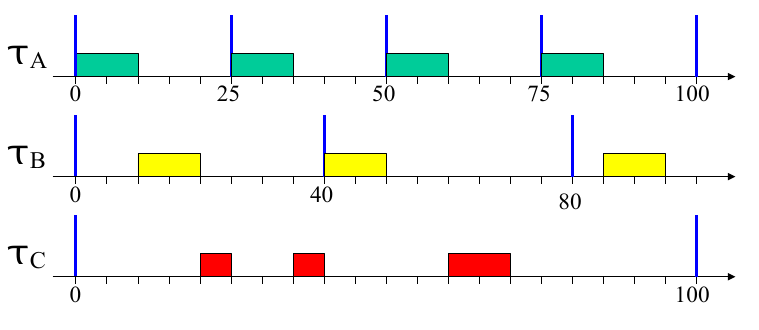
\includegraphics[width=0.5\textwidth]{img/rm_1}
\end{figure}
\\
Definiamo l'utilizzazione della \textit{CPU} da parte di un task come $U_i = \frac{C_i}{T_i}$, in questo modo possiamo andare a calcolare l'utilizzazione della \textit{CPU} su tutti i task definiti:
\begin{center}
    \[U_p = \sum_{i = 1}^{n} \frac{C_i}{T_i} \qquad \leftarrow U_p \text{ processor load} \]
\end{center}
In questo modo riusciamo a valutare il \textbf{carico del processore} che però \textbf{non} è una condizione \textbf{sufficiente} per garantire la \textbf{\textit{schedulabilità}} di un \textit{task set}, ma solo \textbf{necessaria}, infatti ci può dire se il \textit{task set} non è schedulabile in quanto $U_p > 1$ indica che il processore è \textit{overloaded}, ma nel caso in cui $U_p < 1$ ci possono essere dei casi in cui il \textit{task set} non può essere schedulato tramite \textit{RM}. \\
È possibile però identificare un punto, noto come $U_{lub}$ [\textit{least upper bound}] tale per cui sia possibile avere un \textbf{test di schedulabilità} sia \textbf{necessario} che \textbf{sufficiente}. Infatti nel caso in cui $U_p \leq U_{lub}$ il \textit{task set} è sicuramente schedulabile tramite \textit{RM}. Mentre nel caso in cui $U_{lub} < U_p \leq 1$ non possiamo dire niente di certo sulla fattibilità del \textit{task set}.
Per \textit{Rate Monotonic} $U_p^{RM} = n \cdot (2^{\frac{1}{n}} - 1)$ quindi avremo che: \[ \lim_{n\to\infty} U_{lub} = \log_2 2\]
Definiamo il \textbf{\textit{Critical Instant}} come l'istante di tempo in cui è presente il \textit{response time} maggiore, è stato dimostrato che equivale, considernado un \textit{task set} $\mathcal{T}$ all'istante in cui arrivano in corrispondenza tutti i task a più alta priorità. \\
Dal punto di vista della schedulabilità un task sporadico può essere considerato come un task periodico e quindi è possibile calcolarsi il suo $U_p$ e confrontarlo con l'$U_{lub}$ del \textit{task set}. \\
\textbf{\textit{Rate Monotonic}} è \textbf{ottimo}, infatti se esiste un assegnamento a priorità fisse che permette la fattibilità di uno \textit{schedule} per un \textit{task set} $\mathcal{T}$ allora l'assegnamento \textit{RM} è fattibile per il \textit{task set} $\mathcal{T}$, al contrario se un \textit{task set} non è schedulabile con \textit{RM} allora non esiste nessun altro assegnamento a priorità fissa che riesca a rendere fattibile la schedulazione del \textit{task set}. \\
\textbf{\textit{Hyperbolic Bound}}: \[ \prod_{i=1}^n (U_i + 1) \leq 2 \qquad \text{vs.} \qquad \sum_{i=1}^n U_i \leq n \cdot (2^{\frac{1}{n}} - 1)\]

\section{Earliest Deafline First}
Ogni \textit{job} riceve una \textit{deadline \textbf{assoluta}} $d_{i,k} = r_{i,k} + D_i$, in ogni istante di tempo il processore viene assegnato al \textit{job} con la \textit{earliest absolute deadline}, con EDF, qualsiasi set di attività può utilizzare il processore fino al 100\%. \\
\textbf{EDF} è \textbf{ottimale} ovvero se esiste uno \textit{schedule} per $\mathcal{T}$ allora \textbf{EDF} genererà uno \textit{schedule} fattibile, viceverse se $\mathcal{T}$ non è schedulabile con \textbf{EDF} allora non sarà schedulabile per nessun altro algoritmo di scheduling.
Nel caso di \textbf{EDF} il test \textbf{necessario} e \textbf{sufficiente} affinché un \textit{task set} sia schedulabile è che $U_p \leq 1$.
\begin{center}
    \begin{tabular}{ c | c } 
        \textbf{EDF} & \textbf{RM} \\
        \textbf{-} è molto più efficente & \textbf{-} è più semplice implementarla su un sistema operativo commerciale \\ 
        \textbf{-} riduce i \textit{context switches} & \textbf{-} è più predicibile durante \textit{overload} \\
    \end{tabular}
\end{center}

\newpage
\section{Task $D_i \leq T_i$}
Andiamo ora a considerare il caso in cui un task $\tau_i(C_i, D_i, T_i)$ ovvero in cui la \textit{deadline} assoluta non coincide con il \textit{request time} ovvero in cui $D_i < T_i$. In questi casi possiamo utilizzare due tipologie diverse di \textit{scheduler}:
\begin{itemize}
    \item \textbf{\textit{fixed priority}}: \textbf{\textit{Deadline Monotonic}} $p_i \propto \frac{1}{D_i}$
    \item \textbf{\textit{dynamic priority}}: \textbf{\textit{Earliest Deadline First}} $p_i \propto \frac{1}{d_i}$
\end{itemize}
\begin{figure}[h]
    \centering
    \begin{minipage}[t]{0.45\textwidth}
        \centering
        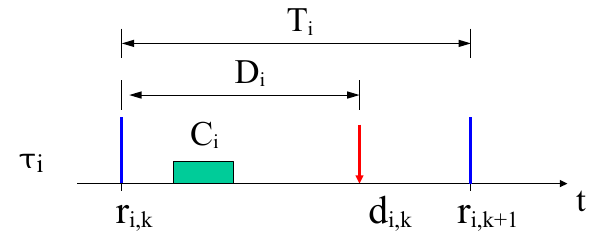
\includegraphics[width=\textwidth]{img/d_less_t_task}
        \caption{\textit{task} con $D_i \leq T_i$}
    \end{minipage}
    \begin{minipage}[t]{0.45\textwidth}
        \centering
        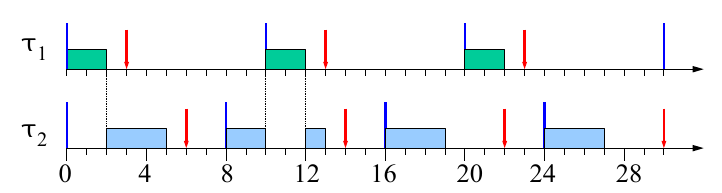
\includegraphics[width=\textwidth]{img/dm_1}
        \caption{\textit{deadline monotonic}}
    \end{minipage}
\end{figure}

\section{Response Time Analysis}
Siccome nel caso di uno scheduler \textit{deadline monotonic} ricavare l'\textit{utilization bound} non è utile in quanto sono fattibili anche \textit{task set} con $U_p > 1$. \\
Il \textit{response time analysis} è un test \textbf{sufficiente} e \textbf{necessario} per la schedulabilità di un \textit{task set} $\tau_i$, per ogni task $\tau_i$ calcolare l'\textit{iterference} $I_i$ che può essere causata da task a più alta priorità, possiamo quindi ora calcolare il \textit{response time} come $R_i = C_i + I_i$ e possiamo verificare che questo sia minore della \textit{deadline} relativa $R_i \leq D_i$. \\
Per calcolare l'interferenza di un task $\tau_k$ (a priorità alta) su $\tau_i$ (a priorità minore) nell'intervallo $[0, R_i]$: \[ I_{ik} \lceil \frac{R_i}{T_k} \rceil \cdot C_k \rightarrow I_k = \sum_{k=1}^{i-1} \lceil \frac{R_i}{T_k} \rceil \cdot C_K \]
Il calcolo del \textbf{\textit{response time}} è invece iterativo:
\begin{center}
    \begin{math}
        \begin{cases}
            R_i^0 = C_i \\
            R_i^{(s+1)} = C_i + \sum_{k=1}^{i-1} \cdot \lceil \frac{R_i^{(s)}}{T_k} \rceil \cdot C_k
        \end{cases}
        \rightarrow R_i^{(s+1)} = R_i^{(s)}
    \end{math}
\end{center}
\newpage
\textcolor{yellow}{\textbf{Esercizio}} \\
Consideriamo un \textit{task set} del tipo:
\begin{math}
    \begin{cases}
        \tau_1 = (3, 6) \\
        \tau_2 = (7, 28) \\
        \tau_3 = (5, 28, 30)
    \end{cases}
\end{math} \\ \newline
andiamo prima a valutare la \textit{schedulabilità} andando a calcolare l'\textit{utiliation bound} modificata, visto che c'è almeno un task che ha $T_i \neq D_i$.
\begin{center}
    \begin{math}
        \begin{aligned}
            U_p^* &= \frac{C_1}{T_2} + \frac{C_2}{T_2} + \frac{C_3}{T_3} \\
            &= \frac{3}{6} + \frac{7}{28} + \frac{5}{28} = 0.93 \qquad \stackrel{\text{?}}{\leq} \qquad U_p^* = n \cdot (\sqrt[n]2 - 1) = 0.78\\
        \end{aligned}
    \end{math}
\end{center}
\begin{itemize}
    \item $\tau_1 \rightarrow R_i = C_i - I_i = 3 - 0 = 3 \stackrel{\text{?}}{\leq} 6$ \textbf{OK}. \\
    Il task $\tau_1$ è \textbf{schedulabile}, siccome siamo in priorità fisse.
    \item il task $\tau_2$ è \textbf{schedulabile}
    \begin{center}
        $R_2 = C_2 + \lceil \frac{R_2}{T_1} \rceil \cdot C_1 = 7 + \lceil \frac{7}{6} \rceil \cdot 3 = 13 \stackrel{\text{?}}{=} 7 \; \mathbf{NO}$ \\
        $R'_2 = 7 + \lceil \frac{13}{6} \rceil \cdot 3 = 16 \stackrel{\text{?}}{=} 13 \; \mathbf{NO}$ \\
        $R''_2 = 7 + \lceil \frac{16}{6} \rceil \cdot 3 = 16 \stackrel{\text{?}}{=} 16 \; \mathbf{SI} \stackrel{\text{?}}{\leq} 28 \; \mathbf{OK}$ 
    \end{center}
    \item il task $\tau_3$ è \textbf{schedulabile}
    \begin{center}
        \begin{math}
            \begin{aligned}
                R_3 &= C_3 +  \lceil \frac{R_3}{T_1} \rceil \cdot C_1  + \lceil \frac{R_3}{T_2} \rceil \cdot C_2 \\
                &= 5 +  \lceil \frac{5}{6} \rceil \cdot 3  + \lceil \frac{5}{28} \rceil \cdot 7 = 15 \stackrel{\text{?}}{=} 5 \; \mathbf{NO} \\
                R'_3 &= 5 +  \lceil \frac{15}{6} \rceil \cdot 3  + \lceil \frac{15}{28} \rceil \cdot 7 = 21 \stackrel{\text{?}}{=} 15 \; \mathbf{NO} \\
                R''_3 &= 5 +  \lceil \frac{21}{6} \rceil \cdot 3  + \lceil \frac{21}{28} \rceil \cdot 7 = 24 \stackrel{\text{?}}{=} 21 \; \mathbf{NO} \\
                R''_3 &= 5 +  \lceil \frac{24}{6} \rceil \cdot 3  + \lceil \frac{24}{28} \rceil \cdot 7 = 24 \stackrel{\text{?}}{=} 24 \; \mathbf{SI} \stackrel{\text{?}}{\leq} 28 \; \mathbf{OK}\\
            \end{aligned}
        \end{math}
    \end{center}
\end{itemize}
Possiamo quindi affermare che l'intero \textit{task set} $\mathcal{T}$ è \textbf{schedulabile}, ed ha una complessità pari a: $\mathcal{O}(n \cdot D_{max})$.
\newpage
\section{Processor Demand Criterion}
In ogni intervallo di tempo la \textit{computation demanded} dal \textit{task set} non deve essere maggiare del tempo disponbiie. Nel caso di \textbf{EDF} abbiamo priorità dinamiche ed è quindi impossibile utilizzare il \textit{response time analysis} per dire se un \textit{task set} è schedulabile. \\
La \textbf{\textit{demand}} in $[t_1, t_2]$ è il \textit{WCET} di quei task che anno $r_i \geq t_1 \cap d_i \leq t_2$: \[ g(t_1, t_2) = \sum_{r_i \geq t_1}^{d_i \leq t_2} C_i\]
Consideriamo ora $t_1 = 0$ (ovvero il \textit{critical istance}) e $t_2 = \mathcal{L}$ e andiamo a calcolarci la \textbf{\textit{demand}} nell'intervallo di tempo $[0, \mathcal{L}]$ allora avremo che: \[g(0, \mathcal{L}) = \sum_{r_i \geq 0}^{d_i \leq \mathcal{L}} C_i = \sum_{i=1}^n \underbrace{\lfloor \frac{\mathcal{L} - D_i + T_i}{T_i} \rfloor}_{\text{Quando i task hanno }r_i\text{ e }T_i \text{all'interno di }\mathcal{L}} \cdot C_i\]
L'\textit{execution time demanded} dai singoli \textit{job} che hanno \textit{deadline} $d_i \leq \mathcal{L}$ su un intervallo di lunghezza $\mathcal{L}$ non può essere maggiore di $\mathcal{L}$ ovvero \[ \forall \mathcal{L} > 0 \; g(0, \mathcal{L}) \leq \mathcal{L} \qquad \leftarrow \text{è inapplicabile } \mathcal{L} \rightarrow \infty \]
\begin{figure}[h]
    \centering
    \begin{minipage}[t]{0.45\textwidth}
        \centering
        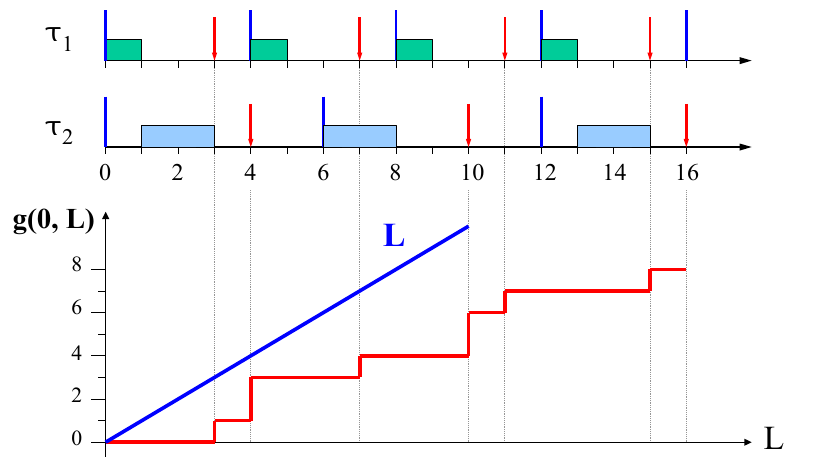
\includegraphics[width=\textwidth]{img/pdc_1}
    \end{minipage}
    \begin{minipage}[t]{0.45\textwidth}
        \centering
        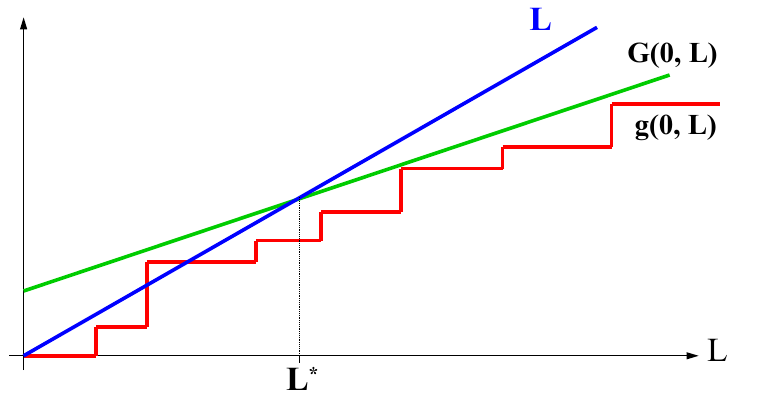
\includegraphics[width=\textwidth]{img/pdc_2}
    \end{minipage}
\end{figure}
\\
Controllare la schedulabilità utilizzando la funzione $g(0, \mathcal{L})$ che è continua nell'intervallo $[0, \mathcal{L}]$ \textbf{non} è \textbf{fattibile}. Possiamo però rendere la funzione un \textit{staircase function} con dei salti (discontinuità) nei punti di \textit{deadline} assoluta $d_{i,k} = (k - 1) \cdot T_i + D_i$, perché possiamo notare dalla figura che i punti in cui la \textit{demand} rischia di superare $\mathcal{L}$ sono nei punti di \textbf{discontinuità}. Possiamo identificare un \textbf{\textit{hyberperiod} H} dopo il quale il comportamento della nostra funzione discontinua si ripeterà, $\mathbf{H} = lcm(T_i, T_j) \; \forall T_i,T_j \in \mathcal{T} \; con \; i \neq j$ ovvero il minimo comune multiplo tra i periodi del \textit{task set}. \\
\[g(0, \mathcal{L}) = \sum_{i=1}^n \lfloor \frac{\mathcal{L} + T_i - D_i}{T_i} \rfloor \cdot C_i\]
\[G(0, \mathcal{L}) = \sum_{i=1}^n (\frac{\mathcal{L} + T_i - D_i}{T_i})  \cdot C_i\]
Per definizione del \textit{floor} avremo che $g(0, \mathcal{L}) \leq G(0, \mathcal{L})$.
\begin{equation}
    \begin{alignedat}{2}
        G(0, \mathcal{L}) &= \sum_{i=1}^n (\frac{\mathcal{L} + T_i - D_i}{T_i}) \cdot C_i \\
        &= \sum_{i=1}^n \frac{\mathcal{L}}{T_i} \cdot C_i + (\frac{T_i - D_i}{T_i}) \cdot C_i \\
        &= \sum_{i=1}^n \mathcal{L} \cdot \underbrace{\frac{C_i}{T_i}}_{U} + (T_i - D_i) \cdot \underbrace{\frac{C_i}{T_i}}_{U_i} \\
        &= \mathcal{L}U \cdot \sum_{i=1}^n (T_i - D_i) \cdot U_i
    \end{alignedat}
\end{equation}
Ora vogliamo trovare il punto di intersezione $\mathcal{L}^*$ tra $\mathcal{L}$ e $G(0, \mathcal{L})$, poniamo quindi: 
\begin{equation}
    \begin{alignedat}{2}
        \mathcal{L} &= G(0, \mathcal{L}) \\
        \mathcal{L} &= \mathcal{L}U \cdot \sum_{i=1}^n (T_i - D_i) \cdot U_i \\
        \mathcal{L} - \mathcal{L}U &= \sum_{i=1}^n (T_i - D_i) \cdot U_i \\
        \mathcal{L} \cdot (1 - U) &= \sum_{i=1}^n (T_i - D_i) \cdot U_i \\
        \mathcal{L}^* &= \frac{\sum_{i=1}^n (T_i - D_i) \cdot U_i}{1 - U}
    \end{alignedat}
\end{equation}
Per verificare quindi se il \textit{task set} è schedulabile dovremo valutare se $\forall \mathcal{L} \in D, \; g(0, \mathcal{L}) \leq \mathcal{L}$ dove avremo che:
\begin{center}
    \begin{math}
        D = \{d_k | d_k \leq \min (\mathbf{H}, \mathcal{L}^*)\}
        \begin{cases}
            \mathbf{H} = lcm(T_i, T_j) \; \forall T_i,T_j \in \mathcal{T}, \; i \neq j \\
            \mathcal{L}^* = \frac{\sum_{i=1}^n (T_i - D_i) \cdot U_i}{1 - U}
        \end{cases}
    \end{math}
\end{center}
\newpage
\textcolor{yellow}{\textbf{Esercizio}} \\
Consideriamo il seguente \textit{task set}: 
\begin{math}
    \begin{cases}
        \tau_1(1, 2, 3) \\
        \tau_2(2, 5.5, 7) \\
        \tau_3(2, 6, 10)
    \end{cases}
\end{math}
\\ \newline
Identifichiamo come prima cosa la nostra $D$: 
\begin{center}
    \begin{math}
        D = \{d_k | d_k \leq \min (\mathbf{H}, \mathcal{L}^*)\}
        \begin{cases}
            \mathbf{H} = lcm(T_1, T_2, T_3) = lcm(3, 7, 10) = 210 \\
            \begin{aligned}
                \mathcal{L}^* &= \frac{\sum_{i=1}^n (T_i - D_i) \cdot U_i}{1 - U} \\ 
                &= \frac{[(3 - 2) \cdot \frac{1}{3}] + [(7 - 5.5) \cdot \frac{2}{7}] + [(10 - 6) \cdot \frac{2}{10}]}{1 - \underbrace{(\frac{1}{3} + \frac{2}{7} + \frac{2}{10})}_{U_{lub} \; = \; 0.8190}} \\
                &= 8.63
            \end{aligned}
        \end{cases}
    \end{math}
\end{center}
\begin{itemize}
    
    \item consideriamo $\mathcal{L} = 2$
    \begin{center}
        $\lfloor \frac{\mathcal{L} + T_1 - D_1}{T_1} \rfloor \cdot C_1 = \lfloor \frac{2 + 3 - 2}{3} \rfloor \cdot 1 = 1 \stackrel{\text{?}}{\leq} 2 \qquad \leftarrow $ \textbf{OK}
    \end{center}
    \item consideriamo $\mathcal{L} = 5$
    \item consideriamo $\mathcal{L} = 5.5$
    \begin{center}
        \begin{math}
            \begin{aligned}
                g(0, \mathcal{L}) &= \lfloor \frac{\mathcal{L} + T_1 - D_1}{T_1} \rfloor \cdot C_1 + \lfloor \frac{\mathcal{L} + T_2 - D_2}{T_2} \rfloor \cdot C_2 \\
                &= \lfloor \frac{5.5 + 3 - 2}{3} \rfloor \cdot 1 + \lfloor \frac{5.5 + 7 - 5.5}{7} \rfloor \cdot 2 \\
                &= 2 + 2 = 4 \stackrel{\text{?}}{\leq} 5.5 \qquad \leftarrow \; \mathbf{OK}
            \end{aligned}
        \end{math}
    \end{center}
    \item consideriamo $\mathcal{L} = 6$
    \begin{center}
        \begin{math}
            \begin{aligned}
                g(0, \mathcal{L}) &= \lfloor \frac{\mathcal{L} + T_1 - D_1}{T_1} \rfloor \cdot C_1 + \lfloor \frac{\mathcal{L} + T_2 - D_2}{T_2} \rfloor \cdot C_2 + \lfloor \frac{\mathcal{L} + T_3 - D_3}{T_3} \rfloor \cdot C_3 \\
                &= \lfloor \frac{6 + 3 - 2}{3} \rfloor \cdot 1 + \lfloor \frac{6 + 7 - 5.5}{7} \rfloor \cdot 2 + \lfloor \frac{6 + 10 - 6}{10} \rfloor \cdot 2 \\
                &= 2 + 2 + 2 = 6 \stackrel{\text{?}}{\leq} 6 \qquad \leftarrow \; \mathbf{OK}
            \end{aligned}
        \end{math}
    \end{center}
    \item consideriamo $\mathcal{L} = 8$
    \begin{center}
        \begin{math}
            \begin{aligned}
                g(0, \mathcal{L}) &= \lfloor \frac{\mathcal{L} + T_1 - D_1}{T_1} \rfloor \cdot C_1 + \lfloor \frac{\mathcal{L} + T_2 - D_2}{T_2} \rfloor \cdot C_2 + \lfloor \frac{\mathcal{L} + T_3 - D_3}{T_3} \rfloor \cdot C_3 \\
                &= \lfloor \frac{8 + 3 - 2}{3} \rfloor \cdot 1 + \lfloor \frac{8 + 7 - 5.5}{7} \rfloor \cdot 2 + \lfloor \frac{8 + 10 - 6}{10} \rfloor \cdot 2 \\
                &= 3 + 2 + 2 = 7 \stackrel{\text{?}}{\leq} 8 \qquad \leftarrow \; \mathbf{OK}
            \end{aligned}
        \end{math}
    \end{center}
\end{itemize}

\resizebox{\textwidth}{!}{%
\begin{forest}
  for tree={
    child anchor=west,
    parent anchor=east,
    grow'=east,
    text width=4cm,
    draw,
    anchor=west,
    edge path={
      \noexpand\path[\forestoption{edge}]
        (.child anchor) -| +(-5pt,0) -- +(-5pt,0) |-
        (!u.parent anchor)\forestoption{edge label};
    },
  }
    [\textbf{Periodic Tasks}
        [\textit{deadline} uguali al periodo: $D_i \stackrel{\text{?}}{=} T_i$
            [\textbf{\textit{Rate Monotonic}}
                [ \textit{optimaily}]
                [ \textit{bounds}
                    [\textit{classical}]
                    [\textit{hyperbolic}]
                ]
            ]
            [ \textbf{\textit{Earliest Deadline First}}
                [\textit{bounds}]
                [\textit{optimaility}]
            ]
        ]
        [\textit{deadline} minore del periodo: $D_i \stackrel{\text{?}}{\leq} T_i$
            [ \textbf{\textit{Deadline Monotonic}}
                [ \textit{per task tests}
                    [\textit{simple}]
                    [\textit{recursive}]
                    [\textit{response time analysis}]
                ]
                [\textit{bounds}]
            ]
            [ \textbf{\textit{Earliest Deadline First}}
                [\textit{processor demand criterion}]
            ]
        ]
    ]
\end{forest}
}


\resizebox{\textwidth}{!}{%
\begin{forest}
  for tree={
    child anchor=west,
    parent anchor=east,
    grow'=east,
    text width=4cm,
    draw,
    anchor=west,
    edge path={
      \noexpand\path[\forestoption{edge}]
        (.child anchor) -| +(-5pt,0) -- +(-5pt,0) |-
        (!u.parent anchor)\forestoption{edge label};
    },
  }
    [ \textbf{RIASSUNTONE}
        [\textbf{Scheduling Approaches}
            [ costruzione offline
                [\textbf{\textit{timeline scheduling}}]
            ]
            [ priorità \textbf{fisse}
                [\textbf{\textit{rate monotonic}}]            
                [\textbf{\textit{deadline monotonic}}]
            ]
            [ priorità \textbf{dinamiche}
                [\textbf{\textit{Earliest Deadline First}}]
            ]
        ]
        [ \textbf{Analysis Techniques}
            [ \textbf{\textit{Processor Utilization Bound}}
                [test \textbf{sufficente}]
                [$U \leq U_{lub}$
                    [$\mathcal{O}(n)$]
                ]
            ]
            [ \textbf{\textit{Response Time Analysis}}
                [test sia \textbf{sufficente} che \textbf{necessario} per \textit{RM} e \textit{DM}]
                [$\forall i \; R_i \leq D_i$
                    [$\mathcal{O}(n \cdot D_{max})$]
                ]
            ]
            [ \textbf{\textit{Processor Demand Criterion}}
                [test sia \textbf{sufficente} che \textbf{necessario} per \textit{EDF}]
                [$\forall \mathcal{L} \; g(0; \mathcal{L}) \leq \mathcal{L}$
                    [\textit{psuedo-polynomial} $U \stackrel{\text{?}}{<}1$]
                ]
            ]
        ]
    ]
\end{forest}
}
